\pagestyle{scrheadings}
\ihead[]{\rightmark}
\ohead[]{Iván Rodríguez Méndez}
\ofoot[]{\thepage{}}
\chapter{Framework experimental}\label{ch:capitulo4}
En esta sección hablaremos de todas las plataformas con las que hemos desarrollado este trabajo.
Entre estas plataformas se encuentran el modelo del robot, el simulador utilizado, programas de diseño y herramientas de cálculo.

\section{Plataforma experimental}
% * <amorellg@ull.edu.es> 2016-06-02T17:41:48.205Z:
%
% > Modelo del Robot
%
% lo llamaría "Plataforma experimental"
%
% ^ <alu0100765755@ull.edu.es> 2016-06-02T18:37:49.984Z.
El robot móvil que hemos decidido utilizar tiene configuración diferencial, es decir, lo que se conoce como robot de interiores.
Este tipo de modelos son más fáciles de guiar a través de la mayoría de trayectorias ya que tiene la capacidad de girar sobre sí mismo.
Por otro lado, la cinemática de este robot es bastante más sencilla que la de un robot que la de un robot en configuración tipo Ackermann (o modelo del triciclo), que permite simplificar la navegación del robot y presentar un caso algo más general.
% * <amorellg@ull.edu.es> 2016-06-02T17:30:20.489Z:
%
% > que la de un robot que implementa el modelo del triciclo lo cual también es una ventaja el hecho de elegir una configuración diferencial.
%
% pondría "que la de un robot en configuración tipo Ackermann (o modelo del triciclo), que permite simplificar la navegación del robot y presentar un caso algo más general."
%
% ^ <alu0100765755@ull.edu.es> 2016-06-02T18:39:42.566Z.
Para llegar a conclusiones más precisas hemos decidido usar un modelo de un robot real, para que así exista la posibilidad de implementar estos algoritmos sobre esta plataforma en un futuro.
Además el Grupo de Robótica de la Univerdad de La Laguna dispone de una unidad (figura \ref{Pioneer_3dx_UNI}), por lo que será factible implementar esto en el futuro sobre el robot real en una continuación de este proyecto o en otro diferente.
\begin{figure}[ht!]
\centering
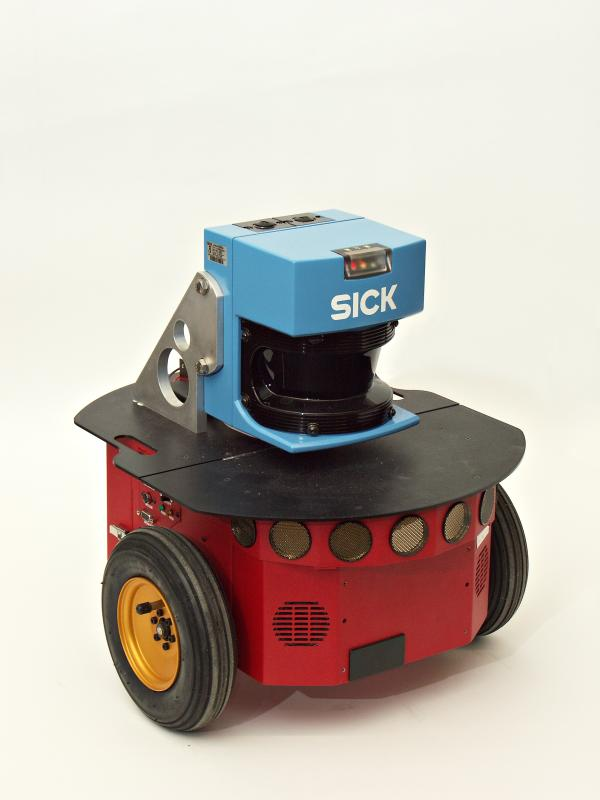
\includegraphics[scale=0.3]{PioneerLaserFront}
\caption{Pioneer P3dx} \label{Pioneer_3dx}
\end{figure}
\begin{figure}[ht!]
\centering
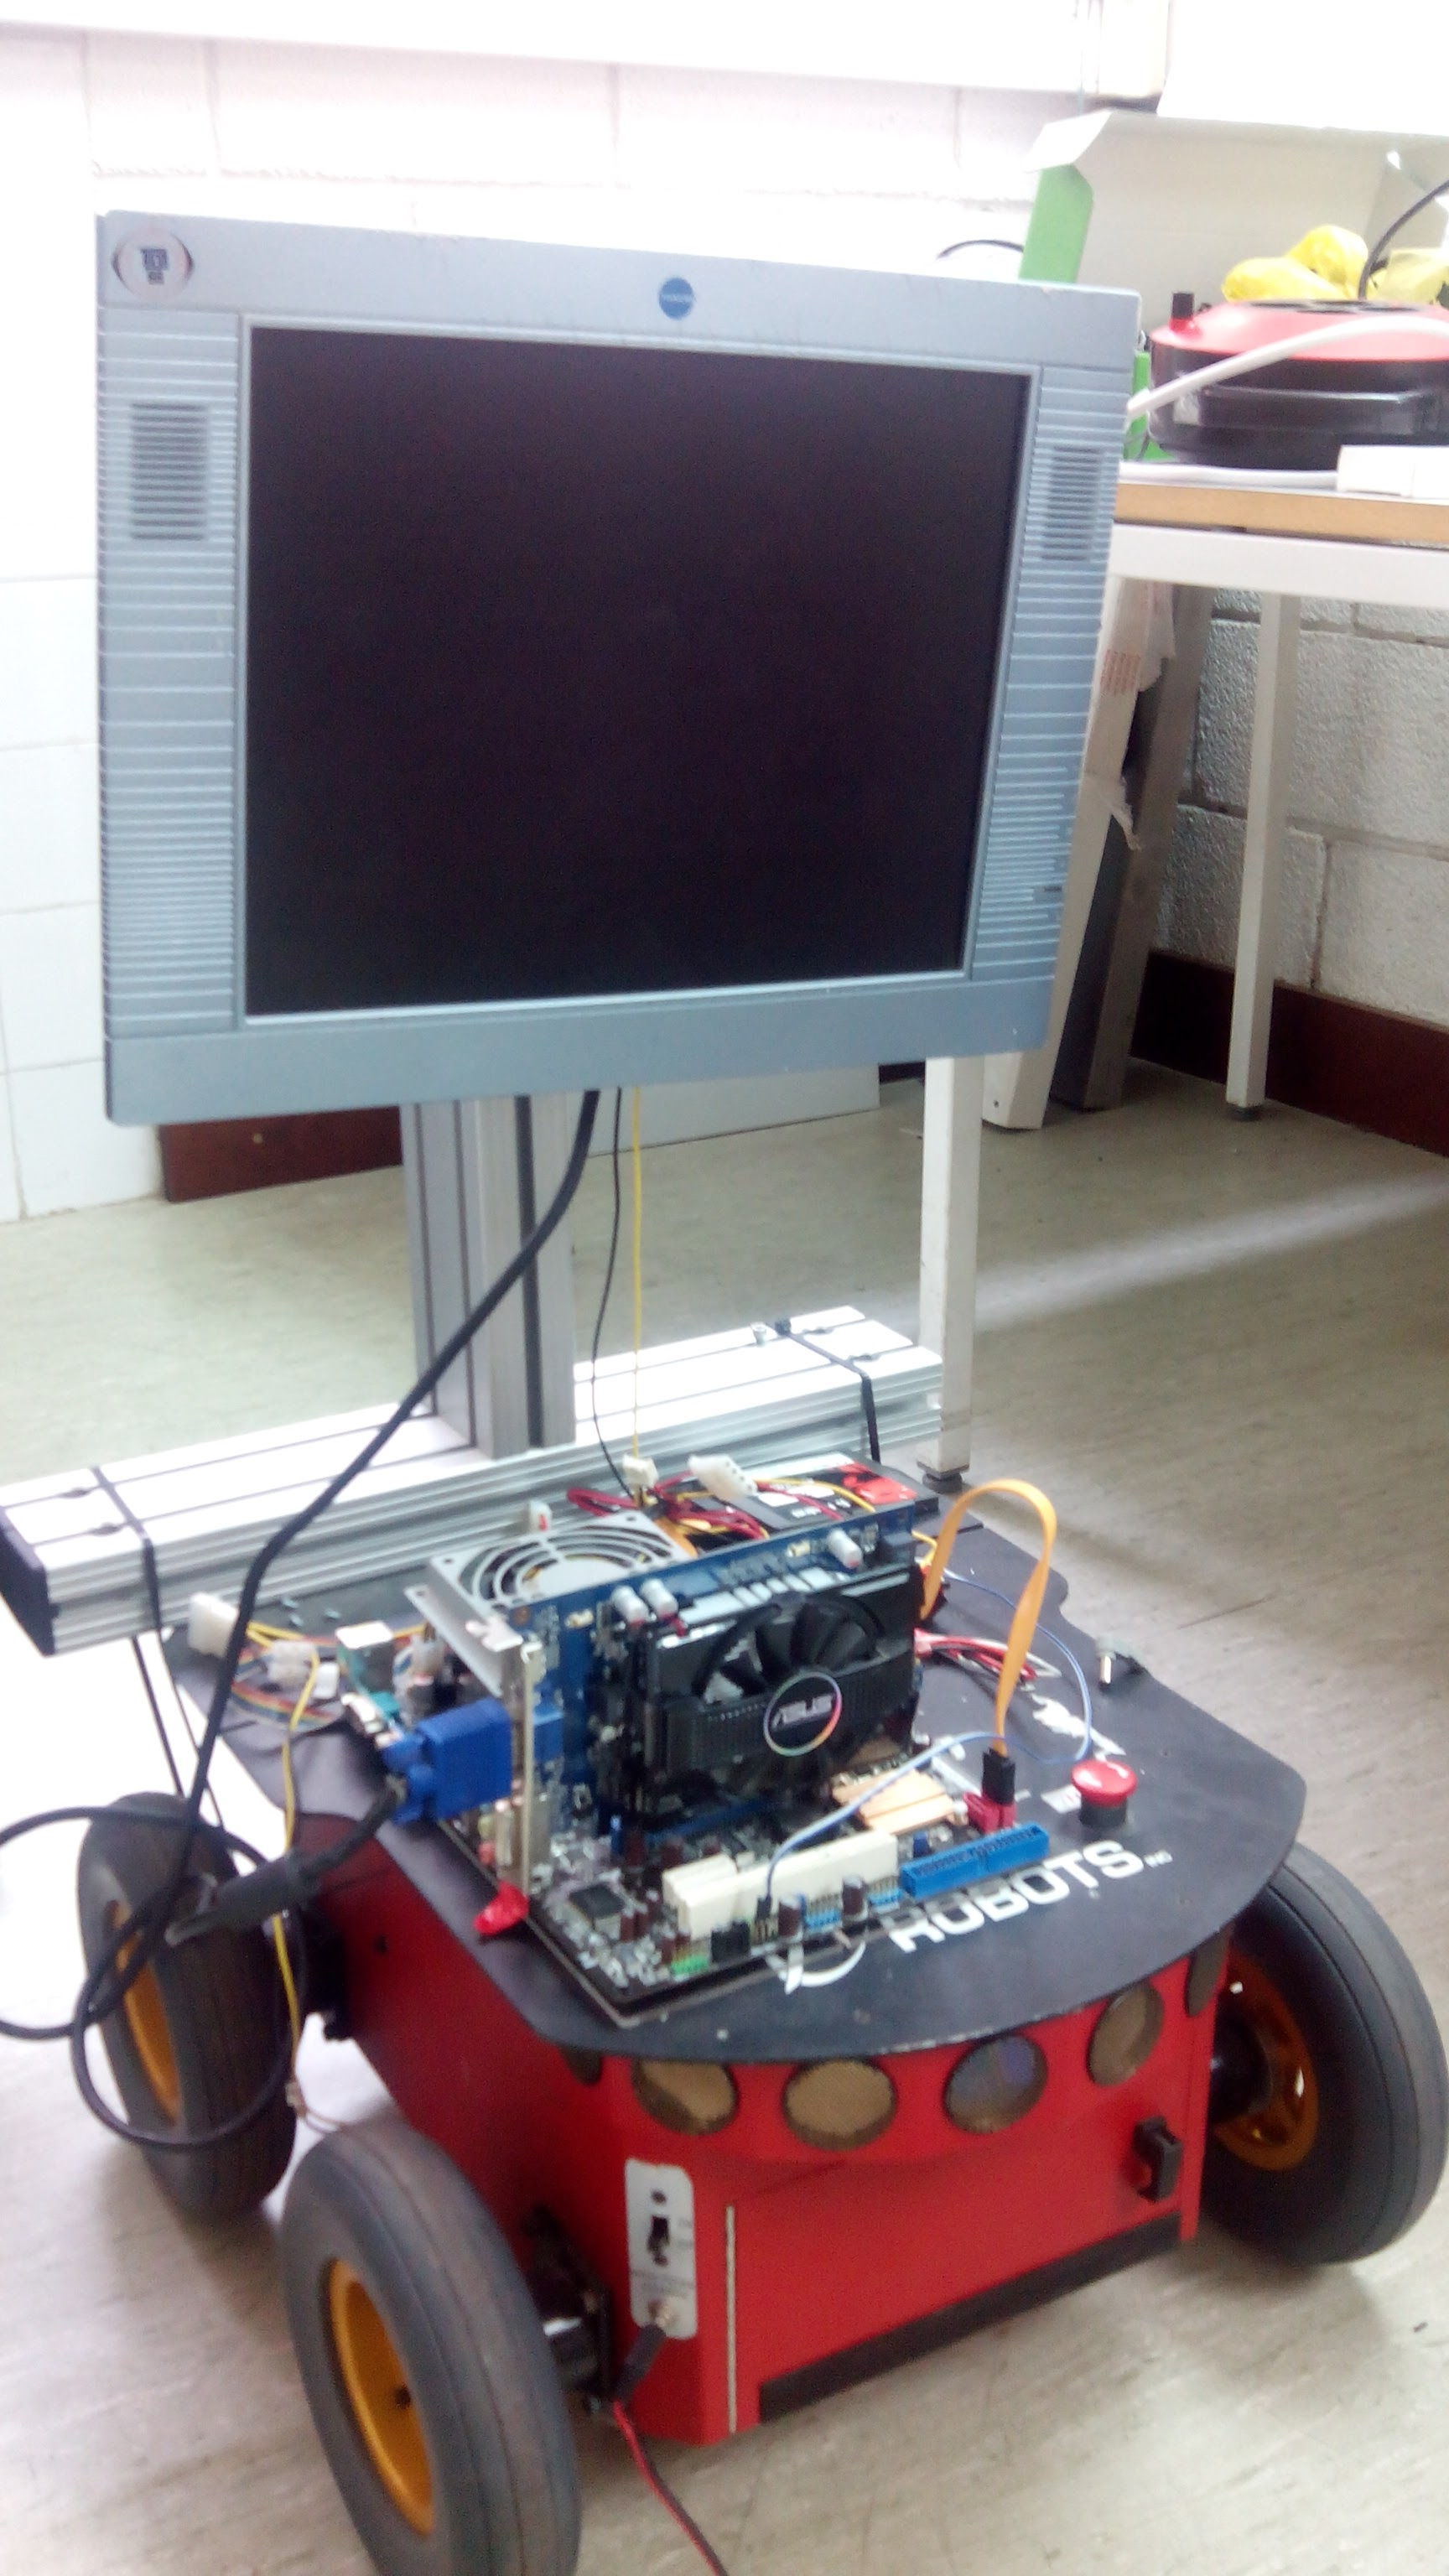
\includegraphics[scale=0.3]{Pioneer_UNI}
\caption{Pioneer P3dx disponible en el GRULL.} \label{Pioneer_3dx_UNI}
\end{figure}
% * <amorellg@ull.edu.es> 2016-06-02T17:32:08.488Z:
%
% > implementar estos algoritmos sobre esta plataforma en un futuro.
%
% añade que el Grupo de Robótica de la Universidad de La Laguna dispone de una unidad, por lo que será factible implementar esto en el futuro sobre un robot real en un proyecto diferente
%
% ^ <alu0100765755@ull.edu.es> 2016-06-02T18:40:58.644Z.

El modelo en concreto que hemos seleccionado es el \textbf{Pioneer P3-DX} \cite{_pioneer_2016} ya que es una de las plataformas más usadas a nivel mundial, es fiable y compacto.
% * <amorellg@ull.edu.es> 2016-06-02T17:31:08.873Z:
%
% > Pioneer 3dx
%
% quizá sea una tontería, pero el nombre correcto del robot es: "Pioneer P3-DX" ----> http://www.mobilerobots.com/ResearchRobots/PioneerP3DX.aspx  Para que lo tengas en cuenta en sucesivas menciones ;)
%
% ^ <alu0100765755@ull.edu.es> 2016-06-02T18:41:21.959Z.
Además tenemos la ventaja de que en el simulador que introduciremos más adelante tiene pre-instalado el modelo.
El sistema sensorial de este robot se compone de encoders ópticos situados en cada eje de motriz, con los que se puede calcular el movimiento mediante \textit{Dead Reckoing }(aplicando el modelo cinemático diferencial) y 16 sensores de ultrasonidos para medir distancias desde el perímetro del robot. Se ha decidido dotar a este modelo de un sensor de profundidad tipo telémetro laser (Sick LMS-100), disponible también físicamente. Este sensor será considerado en las simulaciones como una fuente fiable para medir las balizas del entorno, asumiendo un modelo de ruido para el mismo, que se detalla a continuación.
El modelo de ruido de este tipo de sensores se distribuye de la misma forma que la Gaussiana que podemos ver en la figura \ref{Modelo_ruido}.
\begin{figure}[ht!]
\centering
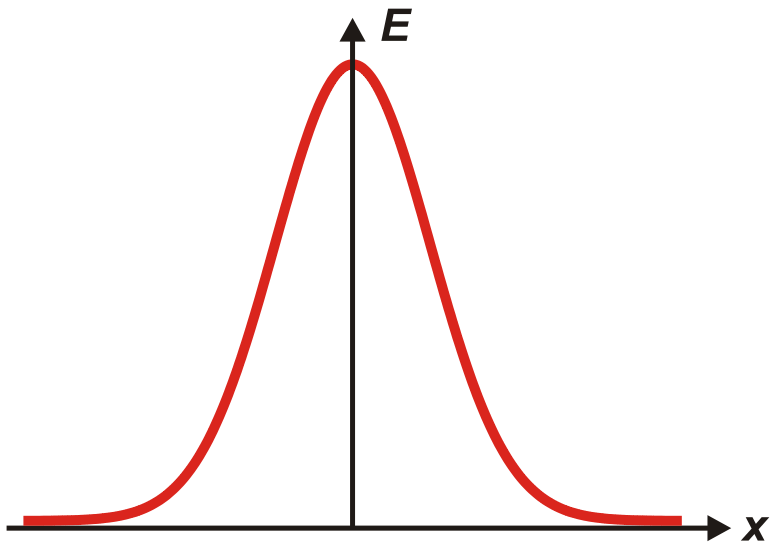
\includegraphics[scale=0.8]{Gaussiana}
\caption{Modelo de ruido sensor.} \label{Modelo_ruido}
\end{figure}
Lo que nos viene a decir esto es que un pulso láser devuelto por los sensores del robot seguirá esta distribución ya que como explicamos en el capítulo \ref{ch:capitulo1} esta es una forma de modelar la certidumbre en los sensores.
Por lo tanto debemos tener en cuenta que la medida devuelta por el sensor tiene un grado de incertidumbre con respecto al valor real de la magnitud que estamos intentando medir.
Cuanto mejor caracterizado tengamos nuestro modelo de ruido mayores nociones tendremos sobre las medidas devueltas por el sensor y su fiabilidad. 

En nuestro caso para la implementación del modelo de medida hemos tenido en cuenta este hecho y para ponerlo de manifiesto en nuestros scripts hemos implementado el modelo de medida de tal manera que aumenta la incertidumbre según nos alejamos.
% * <amorellg@ull.edu.es> 2016-06-02T17:33:58.143Z:
%
% > Este robot puede realizar el cálculo de la odometría gracias a los codificadores de sus ruedas y para realizar medidas del entorno posee 16 sensores de ultrasonidos rodeando el chasis, aunque en el modelo que usaremos en simulación utilizamos un telémetro láser.
%
% lo pondría "El sistema sensorial de este robot se compone de encoders ópticos situados en cada eje de motriz, con los que se puede calcular el movimiento mediante Dead Reckoing (aplicando el modelo cinemático diferencial) y 16 sensores de ultrasonidos para medir distancias desde el perímetro del robot. Se ha decidido dotar a este modelo de un sensor de profundidad tipo telémetro laser (Sick LMS-100), disponible también físicamente. Este sensor será considerado en las simulaciones como una fuente fiable para medir las balizas del entorno, asumiendo un modelo de ruido para el mismo, que se detalla a continuación." Y aquí poner una pequeña explicación del modelo del ruido, a ser posible con una grafiquita pequeña de una gaussiana unidimensional, para explicar que un pulso láser devolverá una medida que seguirá esa distribución.
%
% ^ <alu0100765755@ull.edu.es> 2016-06-02T18:48:11.284Z:
%
% Madre mía , yo no se ni que podría poner para eso jajaja
%
% ^ <alu0100765755@ull.edu.es> 2016-06-02T18:48:13.473Z.


Este robot puede alcanzar velocidades de hasta 1.6$\frac{m}{s}$ y es capaz de soportar una carga de hasta 17 kilos.
Por último, el robot dispone de su propia interfaz de programación, lo que facilita mucho la tarea de pasar el código desde el simulador a la plataforma real.
En la figura \ref{Pioneer_3dx} podemos ver el aspecto que tendría nuestro modelo según la implementación que hemos comentado y en la figura \ref{Pioneer_3dx_UNI} la unidad de la que disponemos.

\section{Modelado 3D usando Blender}
% * <amorellg@ull.edu.es> 2016-06-02T17:42:21.764Z:
%
% > Programas de diseño 3D. Blender
%
% lo llamaría "Modelado 3D usando Blender"
%
% ^ <alu0100765755@ull.edu.es> 2016-06-02T22:21:50.533Z.
Hemos utilizado un programa de diseño tridimensional, en este caso Blender, para realizar los diseños previos de nuestro Robot y así poder modificar cualquier aspecto constructivo por si fuera necesario en el modelo usado por el simulador. 
La idea es realizar el modelo 3D de nuestro robot para disponer de él en el caso de querer extender el diseño constructivo del mismo en el futuro, es decir, nos da la posibilidad de añadir más características constructivas y modificaciones sobre el modelo comercial.
Por otra parte disponer del modelo parametrizado también nos permite poder fabricar recambios para nuestro robot con ayuda de una impresora 3D.% * <amorellg@ull.edu.es> 2016-06-02T17:42:49.084Z:
%
% > Hemos
%
% Aquí (o al final) añadiría como idea fuerte de hacer el modelo 3D en Blender es más bien disponer de él para extender el diseño constructivo del mismo en el futuro. Decir que permite presentar el robot de forma más precisa y eso está bien, no quites nada, pero yo añadiría esto para justificar con más peso el haber hecho un modelo que ya te da V-REP ;)
%
% ^ <alu0100765755@ull.edu.es> 2016-06-02T22:27:06.401Z.
Blender es un programa informático multi-plataforma (además de ser software libre), dedicado especialmente al modelado, iluminación, renderizado, animación y creación de modelos tridimensionales. También puede ser utilizado para la composición digital utilizando la técnica procesal de nodos, edición de vídeo, escultura (incluye topología dinámica) y pintura digital. En Blender, además, se puede desarrollar vídeojuegos ya que posee un motor de juegos interno \cite{_blender_2016}.

Por otra parte el realizar el diseño de nuestro modelo en este programa nos permite presentar el robot de una forma más precisa pudiendo prestar atención a cada detalle de la construcción de este.
\begin{figure}[ht!]
\centering
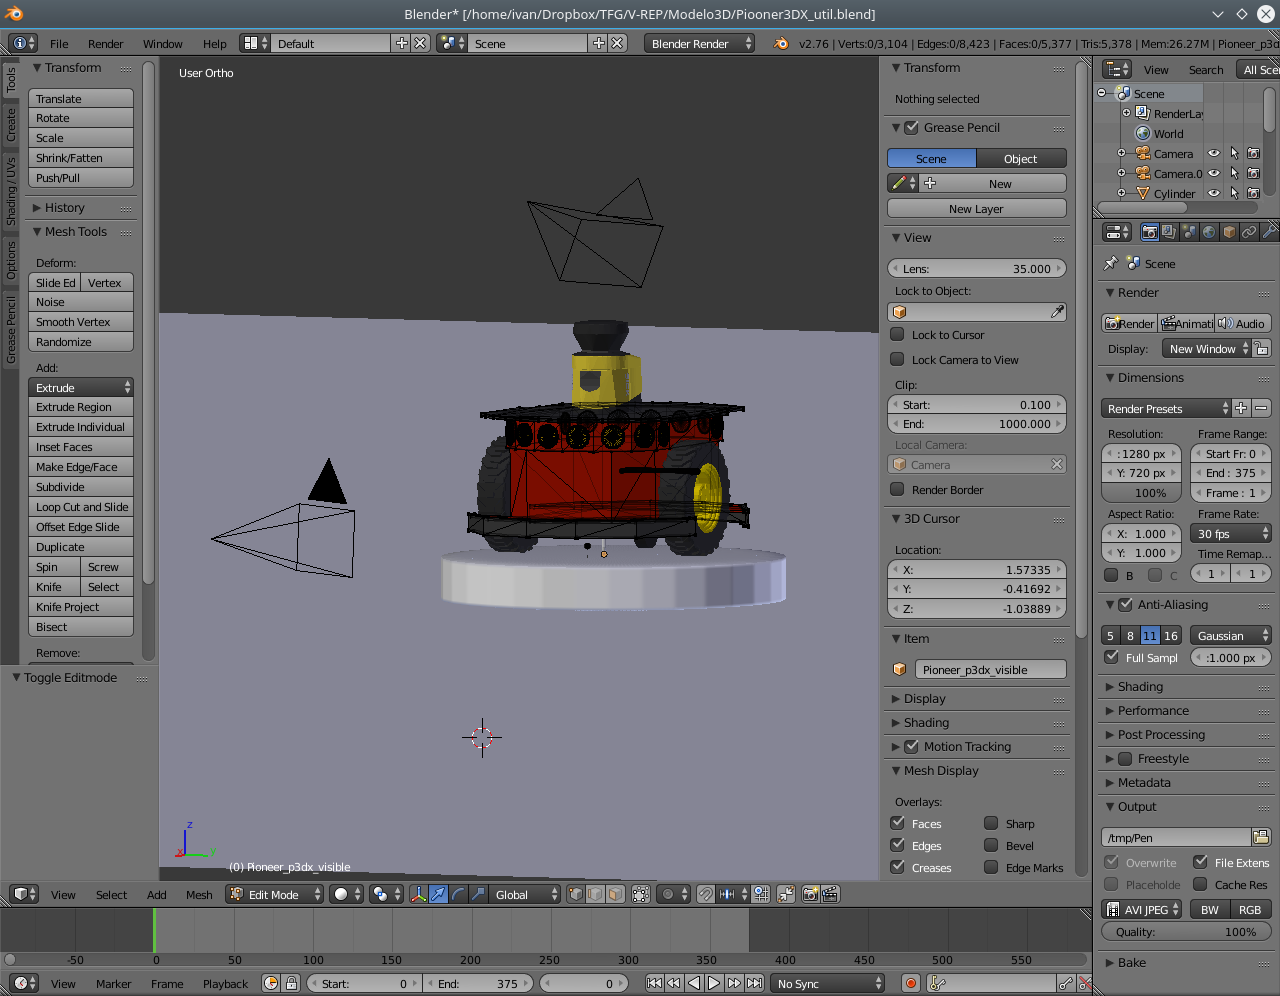
\includegraphics[scale=1]{PioneerBlender}
\caption{Pioneer P3dx en Blender.} \label{Pioneer_3dx_Blender}
\end{figure}
El modelo que podemos ver en la figura \ref{Pioneer_3dx_Blender} es el que posteriormente hemos implementado en V-REP para realizar las simulaciones que estimemos oportunas.
Por último para realizar una presentación más vistosa de nuestro trabajo este programa nos permite realizar animaciones 3D con muy buenos resultados y  exportables en cualquier formato de vídeo.

\section{Simulación dinámica con V-REP}
% * <amorellg@ull.edu.es> 2016-06-02T17:44:52.898Z:
%
% > Plataforma de simulación. V-rep
%
% lo cambiaría por "Simulación dinámica con V-REP"
%
% ^ <alu0100765755@ull.edu.es> 2016-06-02T22:27:54.678Z.
V-REP es programa multiplataforma y además libre que sirve para simular todo tipo de sistemas robóticos \cite{_v-rep._2016}.
Los sistemas que pueden ser estudiados en esta plataforma van desde manipuladores antropomórficos, cadenas de montaje y también disponen de una gran cantidad de modelos de robótica móvil, podemos ver el simulador en la figura \ref{V-REP}.
\begin{figure}[ht!]
\centering
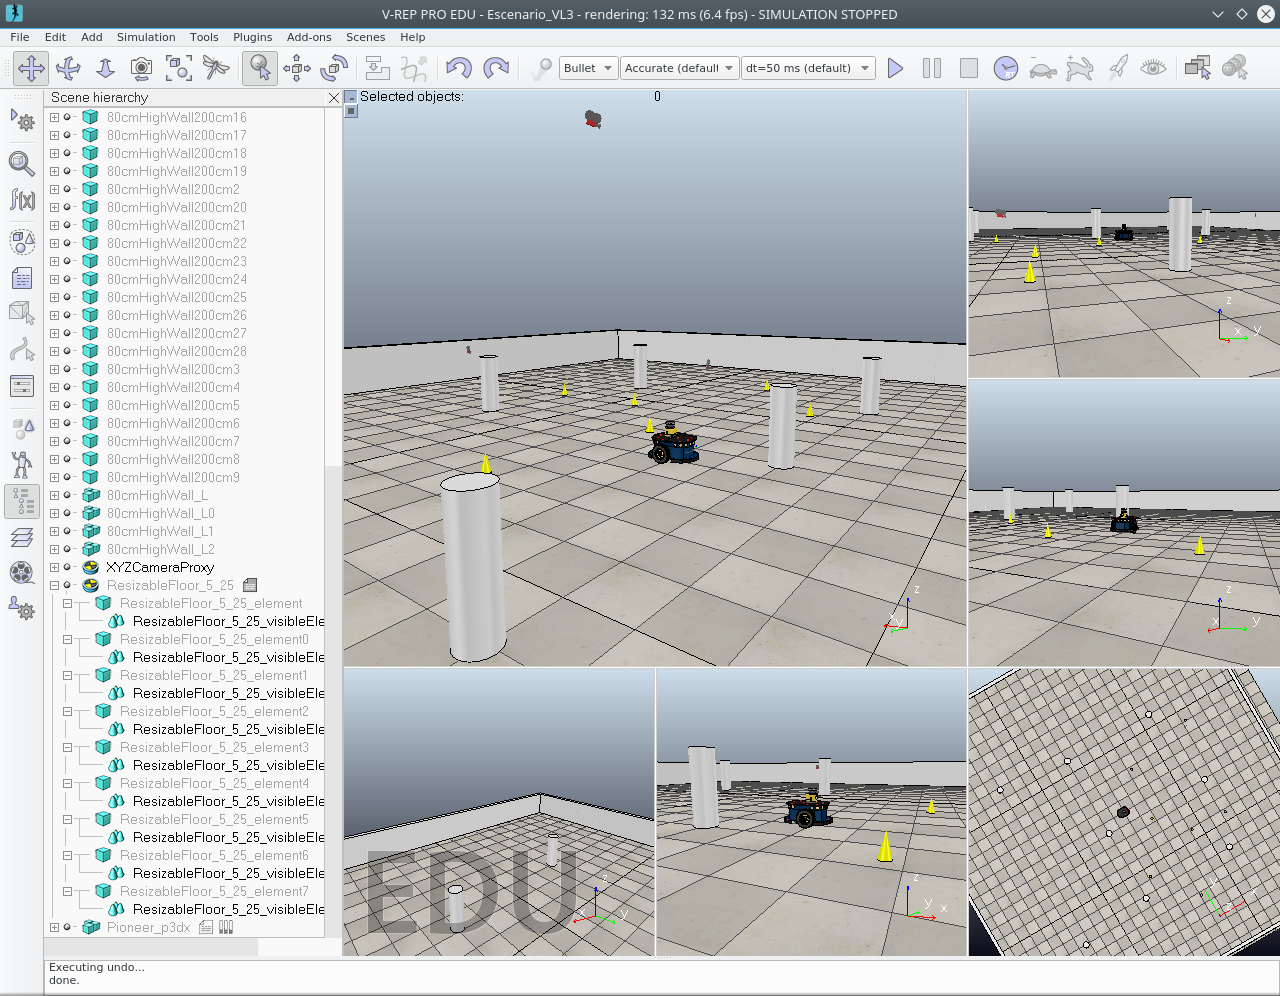
\includegraphics[scale=1]{V-REP}
\caption{Simulación en V-REP.} \label{V-REP}
\end{figure}
Este programa dispone de un motor para interpretar y simular condiciones reales incluyendo físicas complejas.
También dispone de funcionalidades para hacer cálculos de cinemática tanto directa como inversa.
Ofrece un motor para gestionar las colisiones y simulaciones de partículas, como por ejemplo, robots que pintan superficies.
Es capaz de simular una gran cantidad de sensores, y en especial destaca por su capacidad de simular sensores de visión, como cámaras.
Además dispone con un motor de generación de rutas y planificación de movimientos, aunque no usaremos ninguno de estos para la realización de este trabajo.
Permite importar una gran cantidad de modelos propios, como por ejemplo los generados en Blender además de permitir modificaciones sobre la escena cuando la simulación está en marcha.

En cuanto a la simulación, V-REP es un simulador que permite un alto nivel de personalización , de hecho cada parámetro de la simulación y del propio entorno es configurable lo que nos permite adaptar las condiciones de simulación como deseemos en cada momento.
Esto es posible gracias a lo que se conoce como una API (Application Programming Interface) que nos permite controlar el simulador desde un programa externo como puede ser MATLAB/Octave, o incluso desde un código escrito en C++, Python, Java y LUA, entre otras.
Por otra parte también puede ser controlado a través de una interfaz para ROS (Robot Operating System) \cite{_ros.org_2016}.
% * <amorellg@ull.edu.es> 2016-06-02T17:46:14.610Z:
%
% > ROS
%
% poner entre paréntesis Robot Operating System, y cita a la web de ROS: http://www.ros.org/
%
% ^ <alu0100765755@ull.edu.es> 2016-06-02T22:45:17.358Z.
El método que utilizaremos para trabajar con el simulador será programarlo en MATLAB y controlar la simulación desde este último.
V-REP también permite trabajar con una estructura cliente-servidor lo cual nos da la posibilidad de realizar la simulación en un equipo mientras otro se encarga de realizar los cálculos, siempre y cuando los dos se encuentren conectados a la misma red.
% * <amorellg@ull.edu.es> 2016-06-02T17:47:26.401Z:
%
% > V-REP 
%
% te lo he corregido un par de veces, pero ojo que has puesto de distintas formas V-REP, V-Rep, V-REp....
%
% ^ <alu0100765755@ull.edu.es> 2016-06-02T22:49:29.213Z.

\section{Control de simulación mediante MATLAB}
% * <amorellg@ull.edu.es> 2016-06-02T17:48:17.449Z:
%
% > Programa de cálculo. Matlab
%
% lo cambiaría por "Control de la simulación mediante MATLAB"
%
% ^ <alu0100765755@ull.edu.es> 2016-06-02T22:51:00.794Z.
La plataforma de MATLAB está optimizada para resolver problemas en ciencia e ingeniería. El lenguaje de MATLAB, basado en matrices, es una forma intuitiva de trabajar con datos y operar con ellos de manera rápida. Los gráficos integrados facilitan la visualización de los datos y la obtención de información a partir de ellos. Una vasta librería de toolboxes preinstaladas permiten empezar a trabajar inmediatamente con algoritmos esenciales para su dominio. Aunque en nuestro caso trabajaremos con una toolbox elaborada específicamente para trabajar con filtros de Kalman en sistemas discretos\cite{toolbox_simo} y que hemos tenido que instalar de forma manual.
Esta toolbox ha sido desarrollada por Simö Särkkä para la implementación de una serie de filtros, sobre todo para trabajar con sistemas discretizados como es nuestro caso con los filtros de Kalman.
% * <amorellg@ull.edu.es> 2016-06-02T17:50:59.313Z:
%
% >  elaborada específicamente para trabajar con filtros de Kalman
%
% sé que pones la cita, pero no estaría de más decir "desarrollada por fulano de tal..."
%
% ^ <alu0100765755@ull.edu.es> 2016-06-02T22:59:42.375Z.
% * <amorellg@ull.edu.es> 2016-06-02T17:49:23.945Z:
%
% > la forma más natural del mundo
%
% loco!!!! no pongas esto ;)
%
% ^ <alu0100765755@ull.edu.es> 2016-06-02T23:01:42.913Z.
% * <amorellg@ull.edu.es> 2016-06-02T17:49:03.729Z:
%
% >  de ingeniería y científicos
%
% "en ciencia e ingeniería"
%
% ^ <alu0100765755@ull.edu.es> 2016-06-02T23:02:16.569Z.
\begin{figure}[ht!]
\centering
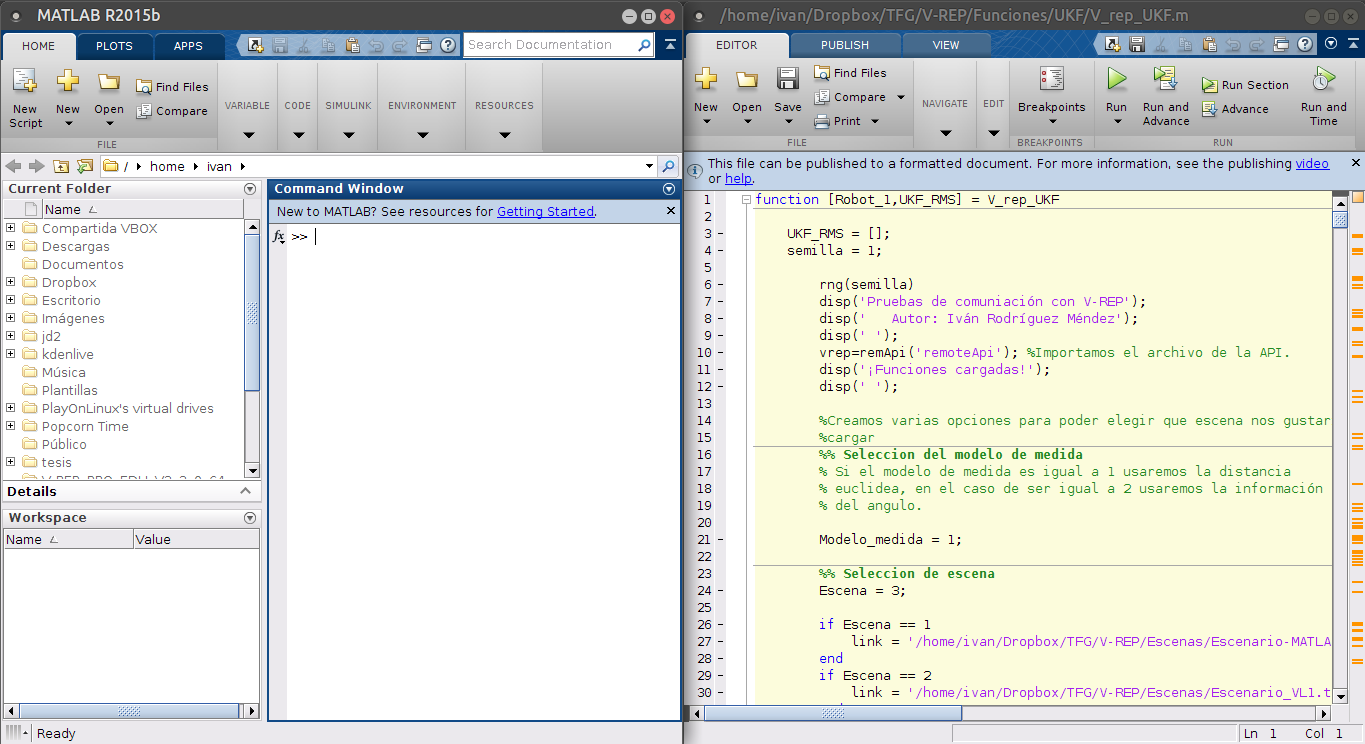
\includegraphics[scale=1]{Matlab}
\caption{Interfaz de Matlab.} \label{Matlab}
\end{figure}
Hemos utilizado MATLAB para realizar todas las simulaciones pertinentes acerca de nuestra implementación del filtro de Kalman en un robot móvil.
% * <amorellg@ull.edu.es> 2016-06-02T17:51:36.008Z:
%
% > Hemos utilizado Matlab para realizar todas las simulaciones pertinentes acerca de nuestra implementación.
%
% Después de esto, para enlazar con lo anterior, especifica qué ofrece la toolbox de serie y qué has desarrollado, para que no parezca que te has limitado a darle a play en los scripts. Esta parte es importante!!! Aquí elabora un poco lo que has tenido que hacer, creando los scripts en donde añades la propagación de la odometría a la estimación y eso
%
% ^ <alu0100765755@ull.edu.es> 2016-06-02T23:38:07.015Z.
Nuestro trabajo con la toolbox  no se ha limitado solamente a ejecutar los códigos que se proporcionan en esta, en el apéndice \ref{ApendiceB} se especifica las funciones que hemos seleccionado para implementar en nuestros scripts .
Nos hemos servido de estas funciones para implementar la localización de nuestro robot, pero antes de realizarla también hemos tenido que desarrollar un entorno en el que poder trabajar en dicha localización.
Hemos creado scripts en los que establecemos una serie de parámetros de simulación para nuestro robot, como pueden ser el ruido del sensor y el deslizamiento de las superficies del entorno y el propio entorno en el que moveremos nuestro robot en V-REP.
Además hemos desarrollado funciones de comunicación, modificación de propiedades de la escena y para la implementación del robot en V-REP (podemos ver todas ellas en el apéndice \ref{ApendiceC}).
Por lo tanto desde MATLAB hemos implementado el control necesario para nuestros experimentos y el robot, la toolbox \cite{toolbox_simo} ha sido una ayuda para no tener que implementar los filtros manualmente en nuestras funciones experimentales y por lo tanto no partir desde cero.

Como un primer paso, hemos realizado simulaciones en dos dimensiones sin conectarnos a V-REP, es decir, realizando todos los cálculos de la cinemática, el trazado de la ruta y la aplicación de los filtros en el código de MATLAB y representándolo por medio de gráficos en 2 dimensiones .
Una vez ya teníamos algunas implementaciones bien configuradas pasamos a escribir el código para una API con V-REP.
Desde MATLAB controlamos todos los parámetros relevantes de la simulación mientras V-REP se encarga de resolver la cinemática de nuestro modelo y los envía a MATLAB para su posterior tratamiento.
Algunos de los parámetros que pasamos entre MATLAB y V-REP son:
\begin{itemize}
\item Velocidad de cada una de las ruedas.
\item Posición del robot real.
\item Posición del robot estimado.
\item Lecturas de los sensores.
\item Posición de los objetivos que el robot debe alcanzar en la escena.
\item Posición de los puntos de referencia o balizas
\end{itemize}
Como vemos hay una gran cantidad de parámetros que se están enviando constantemente entre MATLAB y V-REP.
Sobre estos datos MATLAB nos permite tratarlos y guardarlos con gran facilidad lo cual es una gran ventaja si queremos trabajar con todos los datos obtenidos a posteriori para estudiarlos y llegar a conclusiones sobre ellos.
En el capítulo \ref{ch:capitulo5} especificaremos en mayor profundidad las funciones implementadas en nuestros scripts y el objetivo de estas.

Para más información acerca de las funciones utilizadas al completo dentro de la toolbox lea el apéndice \ref{ApendiceB}.
Si quiere saber más acerca de las funciones que hemos implementado para trabajar con el simulador y la API de V-REP lea el apéndice \ref{ApendiceC}.


